\documentclass[11pt,a4paper]{article}
\usepackage[utf8]{inputenc}
\usepackage[T1]{fontenc}
\usepackage[english]{babel}
\usepackage{lmodern}
\usepackage[margin=2.3cm]{geometry}
\usepackage{amsmath,amssymb,amsthm}
\usepackage{graphicx}
\usepackage{booktabs}
\usepackage{siunitx}
\usepackage{xcolor}
\usepackage{hyperref}
\usepackage{float}
\usepackage{microtype}

\newcommand{\todo}[1]{\textcolor{red}{[TODO: #1]}}
\newcommand{\nside}{N_{\mathrm{side}}}

\title{HWW3: multi-resolution HEALPix unstructured grids for WAVEWATCH III}
\author{Jean-Marc Delouis, CNRS / Grid4Earth}
\date{Internal note, draft of \today}

\begin{document}
\maketitle

\begin{abstract}
We build unstructured WAVEWATCH III (WW3) grids whose nodes are the centres of
HEALPix cells of different resolutions: fine near the coast, coarse in the
open ocean. The model code is unchanged. Because every node is a NESTED
HEALPix pixel, the model state is a multi-resolution HEALPix map. It can be
stored as GRID4EARTH Zarr datasets and compared with satellite products on
the same grid without interpolation. This note describes the grid
construction, how it is validated, and a first North Atlantic simulation for
January 2026. \todo{results}
\end{abstract}

\section{Motivation}
Unstructured wave models usually rely on meshes from generic mesh
generators. Their nodes do not belong to any global indexing system, so every
comparison with observations or with another model needs an interpolation.
HEALPix offers a hierarchical, equal-area and iso-latitude tessellation of
the sphere. Each cell at $\nside$ splits into four cells at $2\nside$, so
multi-resolution grids come from simple quadtree refinement, and each node
has a global integer identifier (the NESTED \emph{uniq} index). Placing the
WW3 nodes at HEALPix cell centres keeps the flexibility of unstructured grids
while making the outputs native to discrete global grid systems.

\section{Grid construction}
\subsection{Refinement}
We start from the cells at $\nside^{\min}$ whose centres lie in the domain,
expanded by a margin. A cell of angular radius $r$ is split into its four
children when its lower-bound distance to the coastline, $d-r$, is below the
distance $D_k$ of a refinement rule $k$ whose target resolution $\nside^{(k)}$
is finer than the cell. The coastline comes from GSHHG (full resolution,
level~1). It is densified to half the finest cell size and thinned to one
point per cell at $4\,\nside^{\max}$. Nearest-coast queries use buckets of
HEALPix cells at $\nside^{\max}/4$, searched by rings of neighbours. The
number of levels is limited to $\log_2(\nside^{\max}/\nside^{\min})\le 4$.

\subsection{2:1 balance}
Leaves are then split until any two leaves sharing an edge \emph{or a corner}
differ by at most one level. A leaf at depth $d$ is split when one of its
eight same-depth neighbours is refined and one of that neighbour's children
is refined as well.

\subsection{Triangulation from the HEALPix adjacency}
Every leaf registers the eight points of its boundary that it can share with
a neighbour: its four corners and the midpoints of its four edges. The
midpoints are the corners of its children. Identical points coming from
different leaves are merged by quantised unit vectors. Around a point $p$,
the registered leaves sorted by angle in the tangent plane at $p$ form a
polygon of cell centres, the dual cell of $p$:
\begin{itemize}
\item 4 cells at a regular vertex;
\item 3 cells at the eight base-face corners where only three cells meet;
\item 3 cells at the midpoint of a coarse edge facing two fine cells.
\end{itemize}
Each maximal run of consecutive wet leaves with at least three members is
triangulated by ear clipping, at each step clipping the ear with the
largest minimum angle.

The mesh is conforming because two leaves sharing a boundary segment
$[p,q]$ are consecutive around $p$ and around $q$ only. Their connecting edge
therefore belongs to exactly the two polygons of $p$ and $q$, and to at most
one triangle in each. With the 2:1 balance, a quarter point of a coarse edge
is registered by at most two fine leaves and never produces a triangle.

\subsection{Ellipsoid}
HEALPix is defined on a sphere. To use the WGS84 ellipsoid, we use the
authalic sphere, which keeps HEALPix equal-area on the ellipsoid. The
geodetic latitudes of all inputs (bathymetry, coastline, domain) are
converted to authalic latitudes before hashing, with the exact formula.
Node latitudes are converted back with a series in $e^2$ refined by two
Newton steps; the round-trip error is below $10^{-12}$\,rad. The difference
between the two latitudes reaches $0.128^\circ$ at $45^\circ$, i.e.\ more
than 14\,km, which is larger than the finest cells. A spherical option is
kept for comparison.

\subsection{Bathymetry and wet cells}
Each GEBCO 2024 sample (15$''$) is assigned to the leaf containing it. A leaf
is wet when at least half of its samples are wet and its mean wet depth
exceeds \SI{5}{m}. The node depth is the mean depth over the wet samples.
Only the largest connected wet component is kept, which removes lakes and
basins not connected to the ocean at the grid resolution.

\section{Validation on synthetic cases}
The mesh is checked automatically: no edge shared by more than two triangles,
no interior edge traversed twice in the same direction, all triangles
counter-clockwise, Euler characteristic $V-E+F = 1-h$ for $h$ holes, and the
largest level jump across an edge. Table~\ref{tab:synth} gives the
multi-resolution test: an island of radius $2^\circ$ centred on a HEALPix
base-face corner ($45^\circ$E, $41.8^\circ$N), with
$\nside = 32\ldots512$ and rules (30\,km, 512), (100\,km, 256), (250\,km, 128).
Figure~\ref{fig:island} shows the mesh around the island.

\begin{table}[H]
\centering
\begin{tabular}{lr}
\toprule
Quantity & Value \\
\midrule
nodes ($\nside$ 32/64/128/256/512) & 94 / 194 / 231 / 297 / 494 \\
triangles & 2471 \\
cells split by the 2:1 balance & 29 \\
non-manifold / inconsistent edges, clockwise triangles & 0 / 0 / 0 \\
Euler characteristic (one island) & 0 \\
max level jump across an edge & 1 \\
min / max angle & \ang{17.0} / \ang{143.7} \\
triangles with an angle $<\ang{20}$ & 1 \\
\bottomrule
\end{tabular}
\caption{Synthetic island test (\texttt{cargo test island\_multiscale}).}
\label{tab:synth}
\end{table}

\begin{figure}[H]
\centering
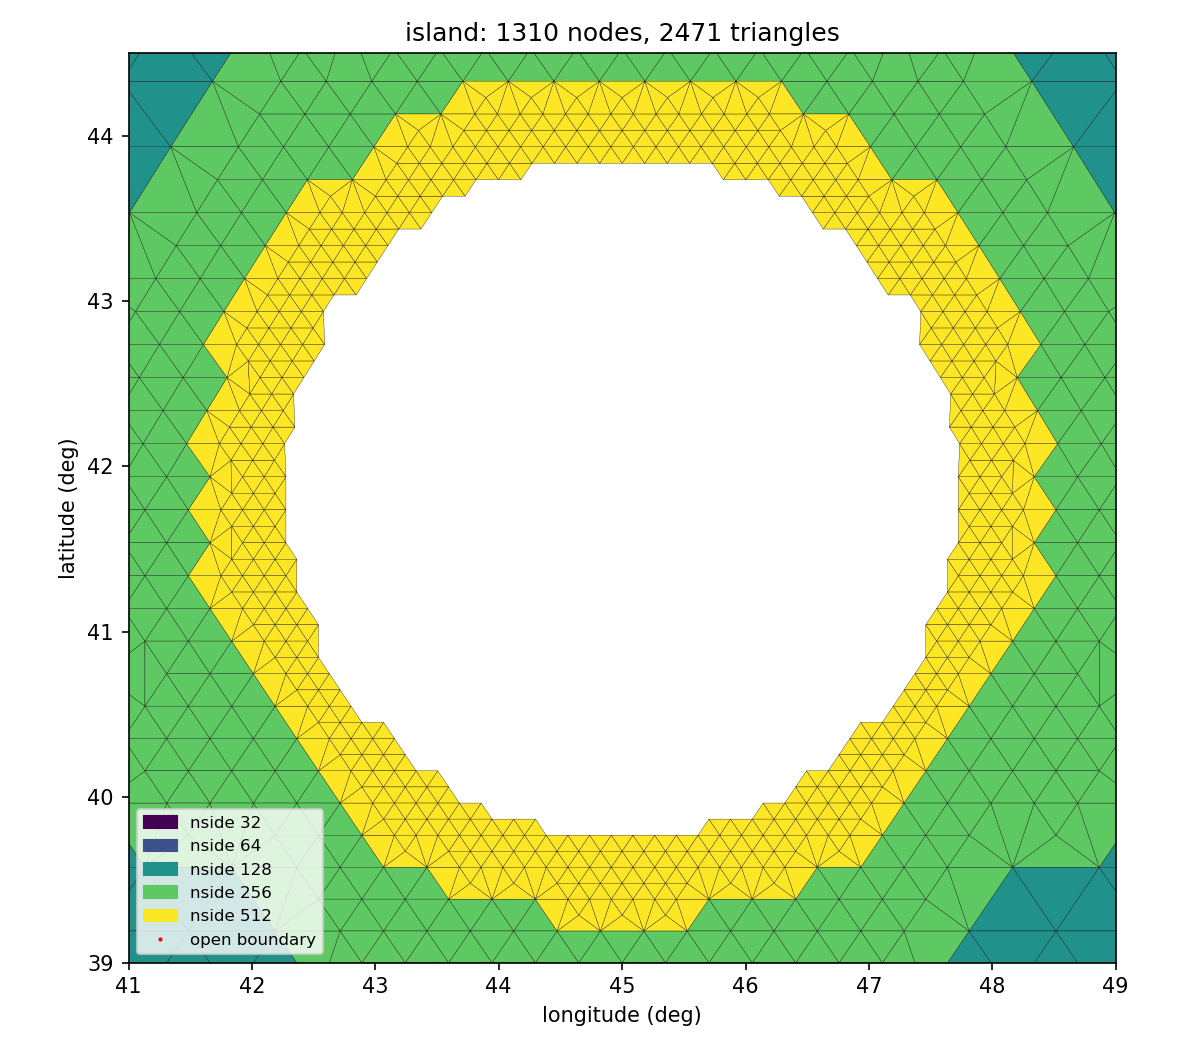
\includegraphics[width=0.75\textwidth]{fig/island_mesh_zoom.png}
\caption{Multi-resolution HEALPix mesh around the synthetic island, coloured
by $\nside$. The island sits on a base-face corner, where only three cells
meet.}
\label{fig:island}
\end{figure}

\section{North Atlantic configuration}
\begin{itemize}
\item Domain: \ang{100}W--\ang{45}E, \ang{0}--\ang{80}N, including the
  Mediterranean and the North Sea.
\item Resolution: $\nside^{\min}=128$ (\(\approx\)\SI{51}{km}) to
  $\nside^{\max}=2048$ (\(\approx\)\SI{3.2}{km}).
\item Refinement rules: \SI{10}{km} $\to$ 2048, \SI{50}{km} $\to$ 1024,
  \SI{200}{km} $\to$ 512.
\item Physics and numerics: WW3 \texttt{develop} (NOAA-EMC), ST4 source
  terms, 36 directions $\times$ 32 frequencies ($f_1=\SI{0.0373}{Hz}$,
  ratio 1.1), implicit unstructured scheme (PDLIB) with domain
  decomposition.
\item Forcing (January 2026): ERA5 10\,m wind; currents and sea level from
  Copernicus Marine; a fixed sea-ice obstruction taken from the January ERA5
  sea-ice concentration.
\item Open boundaries (southern boundary at the equator, eastern Barents
  Sea): spectra from an existing global run. \todo{source of the spectra}
\end{itemize}
\todo{grid statistics, run cost on Datarmor, validation against altimetry}

\appendix
\section{Reproducing}
\begin{itemize}
\item Table~\ref{tab:synth}: \texttt{cd hww3-grid \&\& cargo test --release island\_multiscale -- --nocapture}.
\item Figure~\ref{fig:island}: \texttt{python scripts/plot\_mesh.py /tmp/hww3\_out\_island tex/hww3/fig/island\_mesh\_zoom.png 41 49 39 44.5}.
\end{itemize}

\end{document}
